\section{Functional Verification}
For functional property verification, NetDice \cite{steffen2020probabilistic} 
has laid the way for verifying reachability between two nodes under failure in a 
probabilistic and efficient manner.
To contextualize our modification, we will briefly describe some parts of 
NetDice's network encoding and exploration algorithm as a prelude to our alteration.
For a more complete complete description of NetDice, please refer to the original 
paper.

\begin{figure}[h]
    \centering
    % \includegraphics[width=0.4\textwidth, trim=0cm 11cm 0cm 5cm]{ex.pdf}
    \includegraphics{../tikz/ex}
    % \includegraphics{ex.eps}
    \caption{Example topology, we want to check the reachability of A to Z}
    \label{fig:ex}
\end{figure}

\subsection{Topology Graph}
In this framework, a network is encoded in an edge-labeled directed graph 
$G_t = (V_t, E_t)$ where $V_t$ represents the nodes in the network and 
$E_t$ represents the functional connectivity between a source and a destination node. 
A physical link is then represented as a pair of symmetrical edges that shares the same source 
and destination node but with opposite direction (e.g. $v_1 \rightarrow v_2$ and $v_2 
\rightarrow v_1$).
A routing protocol is then defined on top of this graph by some auxilary information.

To explain it with further clarity, we use the topology in Fig. \ref{fig:ex} as a 
running example for this paper. 
We will assume that the nodes in the network runs OSPF with weight 1 for every edge and ECMP 
as their load-balancing scheme.
We want to check the temporal probability of packets that departs from A to Z.

% To represent the component's random failure, NetDice defined two failure rates.
% The first failure rate is the chance that a given physical link in the network will go down.
% The second failure rate is the chance that a given node in the network will go down.
% These rates are shared between all links / nodes in the network.
% Internally however, the node failure rate will be translated into the link failure rate 
% with a Bayesian Network model, since a node failure can be modeled with the failure of each 
% links connected to it.

To represent random failure, NetDice defined a universal link failure rate (i.e. 
the probability of \textit{any} link in the network randomly failing).
We refine NetDice's model slightly by allowing each links to have different failure rate.
We label each edge in $E_t$ with a function $r: E_t \rightarrow \{x \in \mathbb{R} \mid 0 \le x 
\le 1\}$ that represents the failure rate of a given physical link.
As a consequence, two symmetrical edges (i.e. two edges that shares the same node pairs but with 
opposite direction) will also share the same failure rate, and will be disabled in a coupled 
fashion.

For the sake of example, in our Fig. \ref{fig:ex} topology, we will assume that each link has a 
10\% chance of failure.

% \subsubsection{Routing}
% On top of this topology, NetDice also defined additional informations that would be used
% by a routing protocol to determine the valid path(s) between two nodes $src, dst \in V_t$ given 
% a particular link failure scenario. 
% These routing informations would also be used by their optimization algorithms to reduce the 
% amount of states that are going to be explored.

% NetDice implemented iBGP and OSPF (with ECMP) routing protocols.
% They encode the relevant routing information by assigning some labels to the vertices or edges
% in the topology.
% In OSPF for example, we define a function $w_{ospf}: E_t \rightarrow \mathbb{N}$ as the edge-label 
% that represents the positive weight of a link.
% They would later be used to compute the convergent paths of a given network state 
% (\ref{verification}).

\subsection{State Exploration}
A \textbf{network state} is defined as a set of failed links.
There are $2^{|E_t|}$ network states in a given network and a brute-force strategy 
would need to explore all of the states to compute the reachability property of a 
node pair in a given network. 
NetDice however, will merge multiple network states into an \textbf{equivalence class}
by marginalizing over \textit{cold edges}, links whose failure is guaranteed not to 
change the convergent path of a highlighted network state.

NetDice will systematically explore many equivalence classes in the network. 
It will start from the equivalence class of a perfect network and will fail certain 
\textit{hot edges} (i.e. edges that are not cold) to explore another equivalence 
class.
While not explicit in its description, NetDice's algorithm will effectively form an 
\textbf{exploration tree}. 

In order to preserve some information that will be used in the temporal verification 
stage, we modify this original exploration algorithm to make it more explicit.
We started by formalizing the notion of Equivalence Classes.
An Equivalence Class $\mathcal{E}$ is defined as a 3-tuple $(U_h, D_h, paths)$.
$U_h$ and $D_h$ refers to a set of hot edges that are up and down respectively.
$paths$ refers to the convergent paths between src-dst pair that is produced by the
control plane when the links in $D_h$ fails.
Unlike the original algorithm, we explicitly store $paths$ in $\mathcal{E}$ so that 
it could be used to for the temporal verification stage.

We then define the Exploration Tree $\mathcal{T}$ as a tree of Equivalence Classes.
At the root, we have an Equivalence Class that corresponds to a perfect network, where 
$paths$ is the path(s) that the control plane will produce given a perfect network 
condition and $U_h = D_h = \emptyset$.
Each Equivalence Class in this tree will have children which have one of its parent's link in 
$paths$ appended to its $D_h$, essentially failing one of the link in the path.
If an Equivalence Class has an empty $paths$, then it would have no children.

To compute the functional probability $P_f$ of a given Equivalence Class, we compute the 
product of the 'up' probability of all the links in $U_h$ and $paths$ and the 
product of the 'down' probability of all the links in $D_h$.

In our running example, we could see the subset of the exploration tree in Fig. 
\ref{fig:tree}. 
We see that in a perfect network ($\mathcal{E}_1$), OSPF will produce $ACZ$ as the 
shortest path between A to Z.  
The probability of this Equivalence Class actually materializing ($P_f$) is $0.81$, 
which is the probability of $AC$ and $CZ$ being up at the same time ($0.9^2$).

In the Equivalence Class where the link $AC$ is failing however ($\mathcal{E}_2$), 
OSPF and ECMP will produce two equaly-weighted paths $ABEZ$ and $ADFZ$.
The probability of this Equivalence Class actually materializing ($P_f$) is $0.053$
($0.9^6 \cdot 0.1$).

After having the algorithm produced $\mathcal{T}$, we then continue to the temporal verification 
stage.